\documentclass{article}
%\usepackage{lipsum}
\usepackage{array}
\usepackage[utf8]{inputenc}
\usepackage[T1]{fontenc}
\usepackage{amsfonts}
\usepackage{amsmath}
\usepackage{amssymb}
\usepackage{amsthm}
\usepackage{hyperref}
\usepackage[serbian]{babel}
\usepackage{graphicx}
\usepackage{verbatim}
\usepackage{hyperref}
\usepackage{caption}
\usepackage{subcaption}
\usepackage{float}
\usepackage{tabularx}
\usepackage{tablefootnote}
\setlength{\extrarowheight}{10pt}

\hypersetup{pdfstartview={XYZ null null 1.44}}

\theoremstyle{definition}
\newtheorem{definicija}{Definicija}[section]
\newtheorem{teorema}{Teorema}[section]
\newtheorem{posledica}{Posledica}[teorema]
\newtheorem{lema}[teorema]{Lema}
\newcommand{\dokaz}[1]{\begin{proof}[Dokaz]#1\end{proof}}
\begin{document}
	
	\begin{titlepage}
		\centering
		{\LARGE\bfseries Mašinsko učenje}
		
		\vspace{1cm}
		
		{\LARGE Klasifikacija emocija iz rečenica korišćenjem velikih jezičkih 
        modela sa LoRA tehnikom fine obrade}
		
		\vspace{2cm}
		
		\vfill
		
		{\large 
			\begin{flushleft}
				autor: Dejan Gjer
				\hfill
				mentor: Miloš Radovanović
			\end{flushleft}
		}
		
		
		\vspace{1cm}
		
		{\itshape Univerzitet u Novom Sadu - Prirodno-matematički fakultet}
		
		\vspace{0.3cm}
		
		31.8.2023.
		
		
	\end{titlepage}
	
	\newpage
	
	\tableofcontents
	
	\newpage
	
	\section{Uvod} \label{uvod}
	
	U ovom radu implementirani su modeli mašinskog učenja za prepozvananje 
    emocija iz rečenica i korišćene su različite tehnike fine obrade 
	(fine-tuning) pretreniranog modela. Za pretrenirani model je korišćen BERT
	\cite{bert} model, a potom je treniran metodom fine obrade, prvo treniranjem
	svih parametara pretreniranog modela, a potom LoRA (Low Rank Adaptation)
	tehnikom \cite{lora} na Emotion skupu podatka \cite{emotion-dataset}. 
	Cilj ovog rada je da uporedi ove dve tehnike 
	fine obrade i sagleda njihove prednosti i nedostatke, na jednom tipičnom
	problemu klasifikacije sekvence.
	
	\section{Skup podataka} \label{skup-podataka}
	Kroz ceo rad korišćen je Emotion dataset, jedan od poznatijih skupova 
	podataka za klasifikaciju rečenica koji je uveden u \cite{emotion-dataset}.
	Podaci su sakupljeni iz Twitter komentara na engleskom jeziku i rečenice su
	razvrstane u šest osnovnih kategorija: sreća, tuga, bes, strah, iznenađenje 
	i ljubav. Skup podataka je podeljen na tri dela:
	\begin{itemize}
		\item trening skup - 16000 instanci, koji se koristi za finu obradu 
		(fine-tuning) modela
		\item validacioni skup - 2000 instanci, koji se koristi za evaluaciju
		modela u toku treniranja i na osnovu ovih rezultata se bira najbolja
		verzija modela tokom treniranja, koja se dalje koristi. 
		Takođe ovaj skup se potom koristi i za odabir hiperparametara modela. 
		\item test skup - 2000 instanci, koji se koristi za završno poređenje rezultata
		odabranih modela i generisanje primera klasifikacije.
	\end{itemize}
	Dataset je već obrađen tako da ne sadrži znakove interkpunkcije i sastoji se
	samo iz malih slova. U tabeli \ref{tab1} možete videti neke od primera iz
	ovog skupa podataka.

	\renewcommand{\arraystretch}{0.8}
	\begin{table}
		\centering
		\begin{tabular}{|| >{\centering\arraybackslash} m{8cm} 
			| > {\centering\arraybackslash} m{2cm} ||} 
			\hline
			Rečenica & Labela \\ [0.5ex] 
			\hline\hline
			i have the feeling she was amused and delighted
			& joy \\
			\hline
			i feel like i have to make the suffering i m seeing mean something 
			& sadness \\
			\hline
			i think it s the easiest time of year to feel dissatisfied
			& anger \\  
			\hline
			i began having them several times a week feeling tortured by the
			hallucinations moving people and figures sounds and vibrations
			& fear \\ 
			\hline
			ive been taking or milligrams or times recommended amount and ive
			fallen asleep a lot faster but i also feel like so funny
			& surprise \\
			\hline
			i talk to dogs as i feel they cannot understand words but they 
			can read emotions and know how to be supportive i decided i 
			should go home & love \\ [1ex]
			\hline 
		\end{tabular}
		\caption{\label{tab1} Primeri instanci iz Emotion skupa podataka}
	\end{table}
	
	\section{BERT model} \label{bert}
	BERT (Bidirectional Encoder Representations from Transformers) \cite{bert}
	je veliki jezički model objavljen 2018. godine. 
	Za razliku od Attention is all you need rada \cite{attention} koji je uveo
	transformer arhitekturu koja se sastoji iz enkoder i dekoder mreže,
	BERT je model koji sadrži samo enkoder slojeve (njih 12) i primarno se 
	koristi u oblasti razumevanja teksta.

	Predstavlja jedan od osnovnih modela ovakve strukture i inspiraciju za 
	mnoge modele koji su se pojavili kasnije (DeBERTa, RoBERTa, itd.). 
	U originalnom radu BERT se koristi u dve veličine:
	\begin{itemize}
		\item osnovna (base) - 12 slojeva, 110M parametara
		\item velika (large) - 24 sloja, 340M parametera
	\end{itemize} 
	U ovom radu koristili smo isključivo model osnovne veličine, a u budućem radu
	bilo bi zanimljivo isprobati iste postavke treninga i na velikom modelu i 
	posmatrati da li dolazi do nekih razlika.

	BERT model je pretreniran na velikom korpusu teskta bez labela na dva 
	zadatka: maskirano modelovanje jezika (MLM) i predikcija sledeće rečenice 
	(NSP). MLM je zadatak u kome se određene reči u tesktu maskiraju, a cilj 
	modela je da na osnovu reči u blizini i konteksta predvidi koje reči su 
	maskirane. NSP je zadatak u kome se modelu proslede dve rečenice, a model 
	treba da predvidi da li se one nadovezuju jedna na drugu u tesktu ili ne.

	Da bi se tekst uneo u ovaj model potrebno je izvršiti tokenizaciju teksta. 
	Ona podrazumeva podelu reči iz teksta na jedan ili više delova po određenom 
	algoritmu. Potom se na osnovu rečnika svih tokena, svaki token mapira na
	jedinstveni ključ iz rečnika. U procesu se dodaju i specijalni tokeni koji 
	predstavljaju početak unosa, separator rečenica, itd.

	Tako predstavljen tekst se onda prosleđuje u model koji se sastoji iz enkoder
	blokova, gde svaki enkoder blok sadrži multi-head attention sloj i feed 
	forward mrežu. Izlaz iz enkodera se prosleđuje na linearni klasifikacioni 
	sloj (glava modela) koji može da se prilagođava problemu koji model rešava 
	i generiše verovatnoće potrebne za dobijanje finalnog rezultata. Arhitektura
	modela je prikazana na slici \ref{bert-slika}.

	\begin{figure}[h]
		\centering
		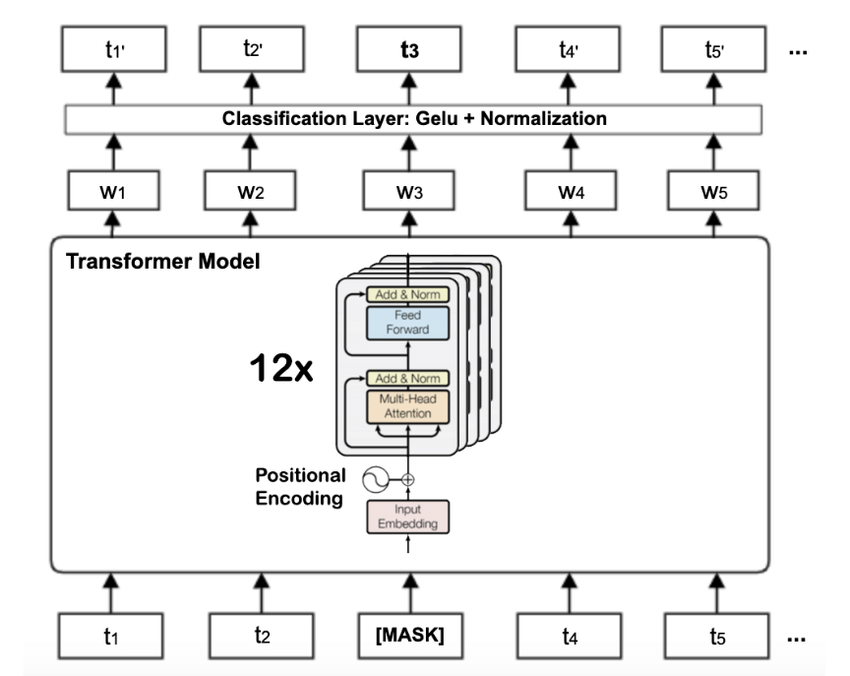
\includegraphics[width=\textwidth]{bert}
		\caption{Prikaz strukture BERT modela \label{bert-slika}}
	\end{figure}

	Pošto BERT model poseduje odlično razumevanje teksta veoma je pogodan za 
	proces finog obučavanja (fine tuning). U ovakvoj postavci treba nam manji 
	skup podataka, sa određenim specifičnim zadatkom (u ovom radu klasifikacija
	emocija) za čije se treniranje koriste pretrenirane težine BERT modela i 
	dodaje odgovarajuća glava modela (obično linearni sloj) koja je nasumično
	inicijalizovana. Pokazalo se da je ovakav oblik učenja transferom mnogo
	efikasniji od treniranja celog modela ispočetka.

	\section{LoRA tehnika} \label{lora}
	LoRA (Low Rank Adaptation) je tehnika za fino obučavanje predstavljena 2021.
	godine u radu \cite{lora}. Motivacija za ovu tehniku se zasniva na 
	pretpostavci da je inherentni rank (intrinsic rank) matrica težina modela 
	koji je fino obučavan veoma mali. Ako označimo težine preobučenog modela sa
	$W$, a $W + \Delta W$ predtavlja težine nakon finog obučavanja, moguće
	je izvršiti dekompoziciju matrice $\Delta W \in \mathbb{R}^{d \times k}$, na 
	dve manje matrice $A \in \mathbb{R}^{d \times r}$ i 
	$B \in \mathbb{R}^{r \times k}$ i $\Delta W = AB$, gde je $r << min(d, k)$ i matrice
	$A$ i $B$ nemaju rank najviše $r$. Rad je pokazao da je
	čak i sa veoma malim vrednostima $r$, umetanjem dekomponovanih matrica
	u model, a zamrzavanjem pretreniranih težina, moguće postići rezultate koji
	su komparativni ili čak i malo bolji od klasičnog pristupa finom obučavanju.
	U LoRA radu izdovojeno je nekoliko prednosti ovakvog pristupa, a među njima su:
	\begin{itemize}
		\item LoRA smanjuje broj trening parametara čak i do 10000 puta u odnosu
		na osnovni model
		\item U slučaju veoma velikih modela (GPT-3 i sl.) moguće je smanjenje
		korišćenja GPU memorije i do 3 puta.
		\item Pretrenirani model može da se fino obučava za više različitih
		zadataka i u tom slučaju za svaki zadatak je dovoljno da čuvamo samo LoRA
		težine (koje zauzimaju mnogo manje skladišta)
	\end{itemize}

	\begin{figure}[h]
		\centering
		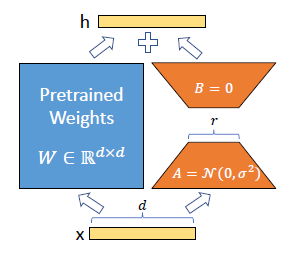
\includegraphics[width=0.35\textwidth]{lora}
		\caption{Prikaz LoRA tehnike \label{lora-slika}}
	\end{figure}

	Cilj ovog rada je da isproba LoRA tehniku finog obučavanja na oblasti
	klasifikacije emocija iz rečenica i da se rezultati i performanse uporede
	sa klasičnim pristupom finog obučavanja.

	\section{Implementacija}
	Za implementaciju ovog projekta korišćen je Python programski jezik uz 
	korišćenje Huggingface API-a za preprocesiranje i treniranje transformer 
	modela, kao i za dodavanje LoRA tehnike. Za praćenje logova i metrika
	eksperimenata, kao i pronalaženje odgovarajućih hiperparametara,
	 korišćen je Weights\&Biases servis. Kod je dostupan na github 
	 repozitorijumu:  \\
	 \url{https://github.com/DejanGjer/Emotion-Classification-LLM-LORA}.

	\section{Postavke treniranja}
	Treniranja se mogu podeliti u dve kategorije:
	\begin{itemize}
		\item Potpuno fino obučavanje (\textbf{FT}) 
		\item LoRA fino obučavanje (\textbf{LORA})
	\end{itemize}
	U obe vrste treniranja korišćen je pretrenirani BERT-base model. Za svaki
	eksperiment kao uslov stajanja, postavljeno je da se model trenira dokle
	god se u četiri uzastopne evaluacije na validacionom skupu podataka ne
	dobije manja tačnost od najbolje postignute do tog trenutka, ili maksimalno
	10 epoha. Tehniku ranog zaustavljanja ovde koristimo da bi se sprečilo
	preobučavanje modela, a takođe se preferira u odnosu na zadavanje 
	konstatnog broja epohi, da bi ispitali da li se uočava razlika u 
	vremenu treniranja do konvergencije u slučaju korišćanja FT tehnike u 
	odnosu na LORU-u.

	Evaluacija na validacionom skupu u toku treniranja se izvršava na
	svakih 250 koraka (što je uvek jedna četvrtina cele epohe). Veličina jednog
	batch-a za sve eksperimente je bila 16 instanci. Na kraju svakog treniranja
	sačuvan je checkpoint modela koji je postizao najveću tačnost na validacionom
	skupu. Optimizator u svim eksperimentima je AdamW sa parametrom $\alpha$
	(koeficijent učenja) koji se podešavao kao hiperparametar i podrazumevanim 
	vrednostima za beta vrednosti ($\beta_1=0.9$, $\beta_2=0.99$). Parametar
	regularizacije $w$ (weight decay) se takođe odabirao kao hiperparametar.
	Takođe u svim treninzima je korišćena ista podela podataka na trening, 
	validaciju i test skupove.

	Za preprocesiranje teksta koristio se BERT-ov tokenizator, gde se svaka rečenica 
	popunjavala (padding) do maksimalne dužine sekvence koju model prihvata.

	Svi treninzi su se izvršavali na PMF-ovom Axiom klasteru, na jednoj Tesla T4
	grafičkoj kartici sa 16GB RAM memorije.

	\subsection{Potpuno fino obučavanje}
	U ovoj postavci birala su se dva hiperparametra: koeficijent učenja $\alpha$
	i parametar regularizacije $w$.	Praćenjem preporukama iz \cite{bert} 
	kao opcije uzete su vrednosti $\alpha \in \{2 * 10^{-5}, 3 * 10^{-5}, 
	5 * 10^{-5}\}$ i $w \in \{0.01, 0.001\}$.

	\subsection{LoRA fino obučavanje}
	U ovoj postavci postoji više hiperparametara od kojih su se neki fiksirali
	na određene vrednosti posle nekoliko preliminarnih eksperimenata, dok su 
	ostali podešavani u eksperimentima koji će kasnije biti prikazani u sekciji
	\ref{rezultati}. Zbog ograničenosti resursa prostor pretrage je morao
	maksimalno da se smanji, pa je moguće da bi se detaljnijom pretragom mogli
	postići bolji rezultati.

	Slede hiperparametri koji su se podešavali. Kao i u FT postavci tu spada
	koeficijent učenja $\alpha \in \{0.0003, 0.001\}$, koji je sada znatno veći,
	nego u prethodnom FT treniranju. Sledeći hiperparametar je dimenzionalnost lora 
	matrica $r$ koju smo objasnili u sekciji \ref{lora}. U radu \cite{qlora} se
	tvrdi kako ovaj parametar ne utiče mnogo na kvalitet rezultata, a u 
	\cite{lora} se ističe kako i veoma male vrednosti, npr. $r=1$, mogu da 
	postignu rezultate ne znatno lošije od onih koje se dosežu sa većim vrednostima. 
	Dakle iako veće vrednosti $r$, pružaju veću dimanzionalnost i broj trening
	parametara, one ne moraju da dovedu do poboljšanja modela. 
	Na osnovu ovih zapažanja izabrano je da $r \in \{2, 8, 32\}$, kako bismo
	ispitali ove tvrdnje u ovom zadatku. Pored toga rad \cite{qlora} navodi kako
	na rezultate više utiče to na koje matrice - slojeve modela će se dekompozicija
	primeniti. Tvrde kako povećanje slojeva koje trenira može da dovede do boljih
	rezultata, više nego parametar dimenzionalnosti $r$. Zbog toga ćemo koristiti
	dve slučaja: u prvom se koriste samo matrice ključa, upita i vrednosti (key, 
	query, value) iz attention blokova, dok u drugom, pored ovih matrica, koriste 
	se i sve iz linearnih slojeva u modelu.

	Faktor skaliranja kod lore (lora $\alpha$) je postavljen na vrednost 16 i po
	preporuci iz \cite{lora} se ne menja za različite vrednosti $r$. Vrednost 
	lora dropout verovatnoće je 0.1 u svim eksperimentima. Takođe je odlučeno
	da kao u \cite{lora}, se ne koriste vrednosti slobodnih članova (bias-a) za
	LoRA parametre.

	\section{Rezultati} \label{rezultati}
	U ovoj sekciji biće prikazani rezultati treniranja modela na dva prethodno 
	objašnjena načina. Prvo ćemo dati pregled 
	metrika koje su korišćene za evaluaciju modela, potom ćemo prikazati 
	rezultate na validacionim skupovima, za sve eksperimente, a na kraju će 
	najbolji modeli biti poređeni na test skupu. Osim toga, pokazaćemo i neke 
	primere tačnih i netačnih predikcija iz test skupa. 

	\subsection{Metrike}
	Eksperimente u ovom radu ćemo porediti na osnovu dve vrste metrika: kvaliteta
	i zauzetih resursa. 
	
	Za metrike kvaliteta, pored funkcije greške treniranja
	(kros entropija), koristićemo i tačnost (accuracy), preciznost (precision),
	odziv (recall) i f1 rezultat (f1 score). Tačnost, kao i inače računa se kao 
	broj tačnih predikcija podeljen brojem ukupnih primera. Sa druge strane, pošto 
	je ovo problem sa više klasa, da bi imali previše metrika za sve klase posebno,
	za preciznost, odziv i f1 rezultat je korišćeno težinsko uprosečavanje. To 
	znači da su ove metrike računate za svaku klasu zasebno, a onda se uprosečene,
	vodeći računa o broju instanci koji pripadaju svakoj klasi. Napominjemo samo
	da su u sekcijama \ref{ft-eval} i \ref{lora-eval} prikazane metrike u koraku
	treniranja koji je davao najbolju preciznost (accuracy) na validacionom 
	skupu podataka, dok su u sekciji \ref{test} prikazane metrike sa test skupa.

	Od metrika zauzeća resursa ispitali smo: vreme izvršavanja (runtime), broj 
	koraka treniranja do konvergencije, prosečno vreme po jednom koraku treniranja,
	maksimalno zauzeće RAM memorije GPU-a i broj trening parametara.
	
	\subsection{Potpuno fino obučavanje} \label{ft-eval}
	
	\begin{table}
		\centering
		\begin{tabular}{| c || c | c | c | c | c | c |} 
			\hline
			& \multicolumn{6}{c|}{Hyperparameters} \\
			\hline
			Learning Rate & \multicolumn{2}{c|}{$2*10^{-5}$} & 
			\multicolumn{2}{c|}{$3*10^{-5}$} & \multicolumn{2}{c|}{$5*10^{-5}$} \\
			\hline
			Weight Decay & 0.001 & 0.01 & 0.001 & 0.01 & 0.001 & 0.01 \\ [0.5ex]
			\hline\hline
			Loss & 0.1926 & 0.1901 & 0.1721 & 0.1723 & 0.2906 & 0.1712 \\
			Accuracy \% & 93.70 & 93.90 & 93.95 & 93.85 & \textbf{94.05} 
			\tablefootnote{Ovaj trening će se u tabeli test rezultata zvati FT} & 93.55 \\
			Precision \% & 94.06 & 94.11 & 94.42 & 94.07 & 94.07 & 93.98 \\
			Recall \% & 93.70 & 93.90 & 93.95 & 93.85 & 94.05 & 93.55 \\
			F1 score  \% & 93.75 & 93.83 & 94.05 & 93.87 & 94.02 & 93.62 \\
			\hline
			Runtime (seconds) & 4572 & 7234 & 5843 & 4523 & 8754 & 4978 \\
			Number of Steps & 2750 & 4000 & 3500 & 2500 & 5250 & 2750\\
			Steps per second & 2.187 & 1.382 & 2.221 & 1.172 & 1.142 & 2.009 \\
			RAM (GB) & 13.4 & 13.4 & 13.4 & 13.4 & 13.4 & 13.4 \\
			Trainable Parameters & 108M & 108M & 108M & 108M & 108M & 108M \\
			Trainable \% & 99 & 99 & 99 & 99 & 99 & 99 \\
			\hline
		\end{tabular}
		\caption{\label{ft-table} Rezultati FT eksperimeneta na validacionom skupu}
	\end{table}

	Na osnovu rezultata iz tabele \ref{ft-table} možemo primetiti da nema velikih razlika u 
	metrikama kvaliteta za izabrane vrednosti hiperparametara. Takođe možemo
	primetiti da su bolje vrednosti na metrikama tačnosti ostvarili modeli koji
	su se izvršavali duže i iterirali kroz veći broj koraka, iako im je funkcija
	gubitka veća u poređenju sa ostalim eksperimentima. To ukazuje na rani početak 
	preobučavanja uprkos idalje odličnim vrednostima metrika na validacionom skupu.

	Metrike koje se odnose na zauzeće resursa (druga grupa), ćemo kasnije uporediti
	sa eksperimentima koji su korisltili LoRA tehniku. Ovde svakako možemo da 
	primetimo da su skoro svi parametri BERT modela trenirajući.

	\subsection{LoRA fino obučavanje} \label{lora-eval}
	Prvo ćemo pogledati rezultate u kojima je LoRA za dekompoziciju koristi samo
	težine iz attention slojeva (tabela \ref{lora-table-att}), a potom rezultate kada koristi i matrice
	težina i iz attention i iz svih linearnih slojeva (tabela \ref{lora-table-lin}).

	\begin{table}
		\centering
		\begin{tabular}{| c || c | c | c | c | c | c |} 
			\hline
			& \multicolumn{6}{c|}{Hyperparameters} \\
			\hline
			$r$ & \multicolumn{2}{c|}{2} & \multicolumn{2}{c|}{8} & 
			\multicolumn{2}{c|}{32} \\
			\hline
			Learning Rate & 0.0003 & 0.001 & 0.0003 & 0.001 & 0.0003 & 0.001 \\ [0.5ex]
			\hline\hline
			Loss & 0.1639 & 0.2462 & 0.1994 & 0.1909 & 0.1444 & 0.2426 \\
			Accuracy \% & 93.85 & 92.30 & \textbf{93.95} 
			\tablefootnote{Ovaj trening će se u tabeli test rezultata zvati 
			LoRA-att} & 93.35 & 93.85 & 92.20\\
			Precision \% & 93.96 & 92.31 & 94.43 & 93.41 & 94.03 & 92.46 \\
			Recall \% & 93.85 & 92.30 & 93.95 & 93.35 & 93.85 & 92.20 \\
			F1 score  \% & 93.87 & 92.29 & 93.99 & 93.27 & 93.86 & 92.27 \\
			\hline
			Runtime (seconds) & 7883 & 3767 & 5169 & 5480 & 7224 & 3093 \\
			Number of Steps & 5750 & 2750 & 3500 & 4000 & 5250 & 2250\\
			Steps per second & 1.269 & 2.654 & 1.935 & 1.824 & 1.384 & 3.234 \\
			RAM (GB) & 11.200 & 11.200 & 11.208 & 11.208 & 11.238 & 11.238 \\
			Trainable Parameters & 83K & 83K & 304K & 304K & 1.189M & 1.189M \\
			Trainable \% & 0.076 & 0.076 & 0.277 & 0.277 & 1.074 & 1.074 \\
			\hline
		\end{tabular}
		\caption{\label{lora-table-att} Rezultati LoRA eksperimeneta sa treniranim 
		parametrima iz attention slojeva na validacionom skupu}
	\end{table}

	\begin{table}
		\centering
		\begin{tabular}{| c || c | c | c | c | c | c |} 
			\hline
			& \multicolumn{6}{c|}{Hyperparameters} \\
			\hline
			$r$ & \multicolumn{2}{c|}{2} & \multicolumn{2}{c|}{8} & 
			\multicolumn{2}{c|}{32} \\
			\hline
			Learning Rate & 0.0003 & 0.001 & 0.0003 & 0.001 & 0.0003 & 0.001 \\ [0.5ex]
			\hline\hline
			Loss & 0.1887 & 0.2929 & 0.1827 & 0.2090 & 0.1681 & 0.1568 \\
			Accuracy \% & 93.95 & 91.20 & \textbf{94.10} 
			\tablefootnote{Ovaj trening će se u tabeli test rezultata zvati 
			LoRA-att+lin}& 92.90 & 93.90 & 93.40 \\
			Precision \% & 94.25 & 91.35 & 94.56 & 93.36 & 94.33 & 93.45 \\
			Recall \% & 93.95 & 91.20 & 94.10 & 92.90 & 93.90 & 93.40 \\
			F1 score  \% & 94.00 & 91.23 & 94.12 & 92.96 & 93.93 & 93.33 \\
			\hline
			Runtime (seconds) & 6252 & 4473 & 5824 & 6227 & 6354 & 8163 \\
			Number of Steps & 3500 & 2500 & 3500 & 3500 & 5250 & 4500\\
			Steps per second & 1.599 & 2.236 & 1.717 & 1.606 & 1.574 & 1.225 \\
			RAM (GB) & 13.930 & 13.930 & 13.958 & 13.958 & 14.066 & 14.066 \\
			Trainable Parameters & 344K & 344K & 1.349M & 1.349M & 5.367M & 5.367M \\
			Trainable \% & 0.313 & 0.313 & 1.217 & 1.217 & 4.673 & 4.673 \\
			\hline
		\end{tabular}
		\caption{\label{lora-table-lin} Rezultati LoRA eksperimeneta sa treniranim 
		parametrima iz attention i linearnih slojeva na validacionom skupu}
	\end{table}

	Poređenjem rezultata iz tabela \ref{lora-table-att} i \ref{lora-table-lin} 
	vidimo da je manja stopa učenja davala bolje rezultate. Vidi se i da je 
	vrednost $r = 8$ u oba slučaja bila najbolja, što je u skladu sa zapažanjima 
	u radu \cite{lora}, ali takođe i da razlike u rezultatima po vrednosti $r$
	nisu veliki. Veću razliku je pravio izbor broja slojeva koji će LoRA trenirati,
	što se opet slaže sa zapažanjima iz \cite{qlora}. Razlika u ove dve tabele
	se primećuje i kod broja i procenta trenirajućih parametara, gde očekivano
	ako LoRA koristi više slojeva, onda i trenira više parametara.

	Ako poredimo FT i LoRA eksperimente, razlike između metrika kvaliteta su 
	izuzetno male, što znači da sa korišćenjem LoRA tehnike nećemo izgubiti
	na kvalitetu istreniranog modela, što je neverovatno ako uporedimo razliku
	u broju treniranih parametara, gde LoRA može da trenira i manje od 1\% 
	parametara koje koristi potpuno fino obučavanje. Vreme koje je potrebno za
	treniranje modela, u obe strategije treninga, kao i broj koraka po sekundama
	se ne razlikuju mnogo. Samim tim u ovom slučaju nisamo uočili da se model
	trenira brže LoRA tehnikom u odnosu na FT. Razlika još može da se primeti 
	u zauzeću memorije grafičke kartice. Ako koristimo LoRA tehniku samo na 
	attention slojevima uspemo da uštedimo više od 2GB memorije. 

	Ova razlika bi bila još veća kada se koriste modeli sa više parametara u 
	odnosu na BERT base model. Ipak, veoma iznenađujuće, kada LoRA tehniku 
	primenimo i na linearne slojeve, alokacija GPU memorije se i poveća u odnosu
	na fino treniranje celog modela (FT). Nismo sigurni šta je uzrok ove pojave,
	moguće je da pošto se ne koriste podrazumevane vrednosti slojeva za primenu
	LoRA-e na BERT modelu, Huggingface frejmvork nije optimizovao takav slučaj.
	Za dalju istragu ove pojave trebalo bi pokušati replicirati takve rezultate
	 i na drugom hardveru.

	\subsection{Rezultati na test skupu podataka} \label{test}
	O ovom poglavlju ćemo prvo prikazati rezultate metrika na test skupu za 
	najbolje eksperimente iz prethodne tri tabele. 

	\begin{table}
		\centering
		\begin{tabular}{| c || c | c | c |} 
			\hline
			& Loss & Accuracy \% & F1 score \% \\
			\hline \hline
			FT & 0.3259 & 93.00 & 92.90 \\
			\hline
			LoRA-att & 0.2220 & 92.25 & 92.27 \\
			\hline
			LoRA-att+lin & 0.2102 & 92.70 & 92.68 \\
			\hline
		\end{tabular}
		\caption{\label{test-table} Rezultati najboljih treninga na test skupu podataka}
	\end{table}

	U tabeli \ref{test-table} dobijamo potvrdu da razlike između ovih pristupa
	nisu velike po metrikama tačnosti i F1 rezultatu. Očekivano, sve metrike su
	malo lošije u odnosu na vrednosti dobijene na validacionom skupu. Slede
	nasumično izvučeni primeri rečenica iz test skupa.

	\begin{table}
		\centering
		\begin{tabular}{|| >{\centering\arraybackslash} m{8cm} 
			| > {\centering\arraybackslash} m{2cm} 
			| > {\centering\arraybackslash} m{2cm} ||} 
			\hline
			Rečenica & Predikcija & Labela \\ [0.5ex] 
			\hline\hline
			i feel so relaxed and happy when im in the water
			& joy & joy\\
			\hline
			i grew up feeling rejected by my male peers 
			& sadness & sadness \\
			\hline
			i feel impatient with brian s prolonged assertion of his alien
			encounter but nobody other than the victim could truly relate
			to repercussion of being molested
			& anger & anger \\  
			\hline
			i still feel scared every time i go into a strange place
			& fear & fear \\ 
			\hline
			i feel more gentle that way wth
			& love & love \\
			\hline
			i feel so weird and scattered with all wonders about a million
			different things
			& fear & surprise \\
			\hline
			i were to go overseas or cross the border then i become a foreigner 
			and will feel that way but never in my beloved land 
			& joy & love\\ [1ex]
			\hline 
			i were to go overseas or cross the border then i become a foreigner 
			and will feel that way but never in my beloved land 
			& joy & sadness \\
			\hline
			i were to go overseas or cross the border then i become a foreigner
			and will feel that way but never in my beloved land
			& surprise & fear \\
			\hline
			i feel so helpless right now
			& sadness & fear \\
			\hline
			i cannot even begin to express in words the depth of sorrow that i
			feel having not posted any of my ludicrous rants over the passed days
			& joy & surprise \\
			\hline
		\end{tabular}
		\caption{\label{inference-tabela-FT} Primeri klasifikacije rečenica na 
		test skupu sa FT modelom}
	\end{table}

	\begin{table}
		\centering
		\begin{tabular}{|| >{\centering\arraybackslash} m{8cm} 
			| > {\centering\arraybackslash} m{2cm} 
			| > {\centering\arraybackslash} m{2cm} ||} 
			\hline
			Rečenica & Predikcija & Labela \\ [0.5ex] 
			\hline\hline
			i say i want to be more of people person but i feel very mellow right now
			& joy & joy\\
			\hline
			i feel like im being really needy
			& sadness & sadness \\
			\hline
			i am not feeling the love towards myself and that becomes somewhat of a vicious
			circle resulting in me just feeling lazy complacent and in general just
			de motivated
			& anger & anger \\  
			\hline
			i feel intimidated by the tasks you feel overwhelmed by huge and
			complicated tasks
			& fear & fear \\ 
			\hline
			i feel more gentle that way wth
			& love & love \\
			\hline
			i feel for all of you who have been supporting me is so extreme there
			would be no way to put a number value on it
			& love & joy \\
			\hline
			i have been sitting at home revising today and all in all feeling quite
			stressed 
			& sadness & anger \\ [1ex]
			\hline 
			i tell you that i love you and my feelings are sincere my dear
			& love & joy \\
			\hline
			i wanted to skate fast wanted to try everything just to see the
			difference in feel which was amazing
			& joy & surprise \\
			\hline
			i will nolonger tell anybody how i feel or what im thinking cause all
			it seems to do is get me more hated than i already am
			& anger & sadness \\
			\hline
			im feeling absolutely amazing
			& joy & surprise \\
			\hline
		\end{tabular}
		\caption{\label{inference-tabela-lora} Primeri klasifikacije rečenica na 
		test skupu sa LoRA-att modelom}
	\end{table}

	Iz ovih primera primećuje se da je neke rečenice veoma teško klasifikovati iako
	da je za neke moguće dodeliti više klasa koje bi imale smisla zavisno od šireg
	konteksta. Oba modela prave slične greške i mešaju slične klase, tako da se 
	ne vidi značajna razlika između njih.

	\section{Zaključak} \label{zakljucak} 
	U ovom radu izvršena je klasifikacija emocija iz rečenica korišćenjem BERT
	modela sa finim obučavanjem celog modela, kao i sa LoRA tehnikom finog 
	treniranja. Analizom rezultata utvrđeno je da BERT model može vrlo uspešno
	da reši ovaj zadatak. Poređenjem ove dve tehnike treniranja nije uočena
	značajna razlika u kvalitetu modela i brzini treninga. Ipak u sitaciji kada
	imamo više specifičnih zadataka, za koje želimo da koristimo isti osnovni 
	model, LoRA je odličan izbor jer postiže slične performanse uz značajno
	smanjenje potrebnog skladišta zbog malog broja dodatnih trening parametara.
	Takođe, LoRA tehnika primenjena na attention slojeve može da smanji količinu
	alocirane memorije od strane grafičke kartice na ovom zadatku. Dobijeni rezultati
	se umnogome poklapaju sa zapažanjma i očekivanjima na osnovu radova \cite{lora} i 
	\cite{qlora}.


	\newpage
	
	\begin{thebibliography}{99}
		%ovde dodati bilo kakve resurse koji se citiraju}
		\bibitem{bert}
        Jacob Devlin and Ming-Wei Chang and Kenton Lee and Kristina Toutanova \\
        \newblock {BERT: Pre-training of Deep Bidirectional Transformers
        for Language Understanding} \\
        \newblock {arXiv:1810.04805}

        \bibitem{emotion-dataset}
        Saravia, Elvis  and
        Liu, Hsien-Chi Toby  and
        Huang, Yen-Hao  and
        Wu, Junlin  and
        Chen, Yi-Shin \\
        \newblock {{CARER}: Contextualized Affect Representations for Emotion Recognition}

        \bibitem{lora}
        Edward J. Hu and Yelong Shen and Phillip Wallis and Zeyuan Allen-Zhu and Yuanzhi Li 
        and Shean Wang and Lu Wang and Weizhu Chen \\
        \newblock {LoRA: Low-Rank Adaptation of Large Language Models} \\
        \newblock {arXiv:2106.09685}

		\bibitem{qlora}
		Tim Dettmers and Artidoro Pagnoni and Ari Holtzman and Luke Zettlemoyer \\
		\newblock {QLoRA: Efficient Finetuning of Quantized LLMs} \\
		\newblock {arXiv:2305.14314}

		\bibitem{attention}
		Ashish Vaswani and Noam Shazeer and Niki Parmar and Jakob Uszkoreit and 
		Llion Jones and Aidan N. Gomez and Lukasz Kaiser and Illia Polosukhin \\
		\newblock {Attention Is All You Need} \\
		\newblock {arXiv:1706.03762}
		
	\end{thebibliography}	
	
\end{document}